%Ambassador
\newcommand{\ambassadorDescription}{
\section{Ambassador}
    Ambassador Text\\
    See \nref{tlttree:ambassador} for more information.
}

\newcommand{\ambassadorTree}{
    \newpage
    \subsection{Ambassador Talent Tree}
    \label{tlttree:ambassador}

    \textbf{Class Skills:} Charm, Discipline, Negotiation, Knowledge (Education), Knowledge (Geography), Leadership
    \newline

    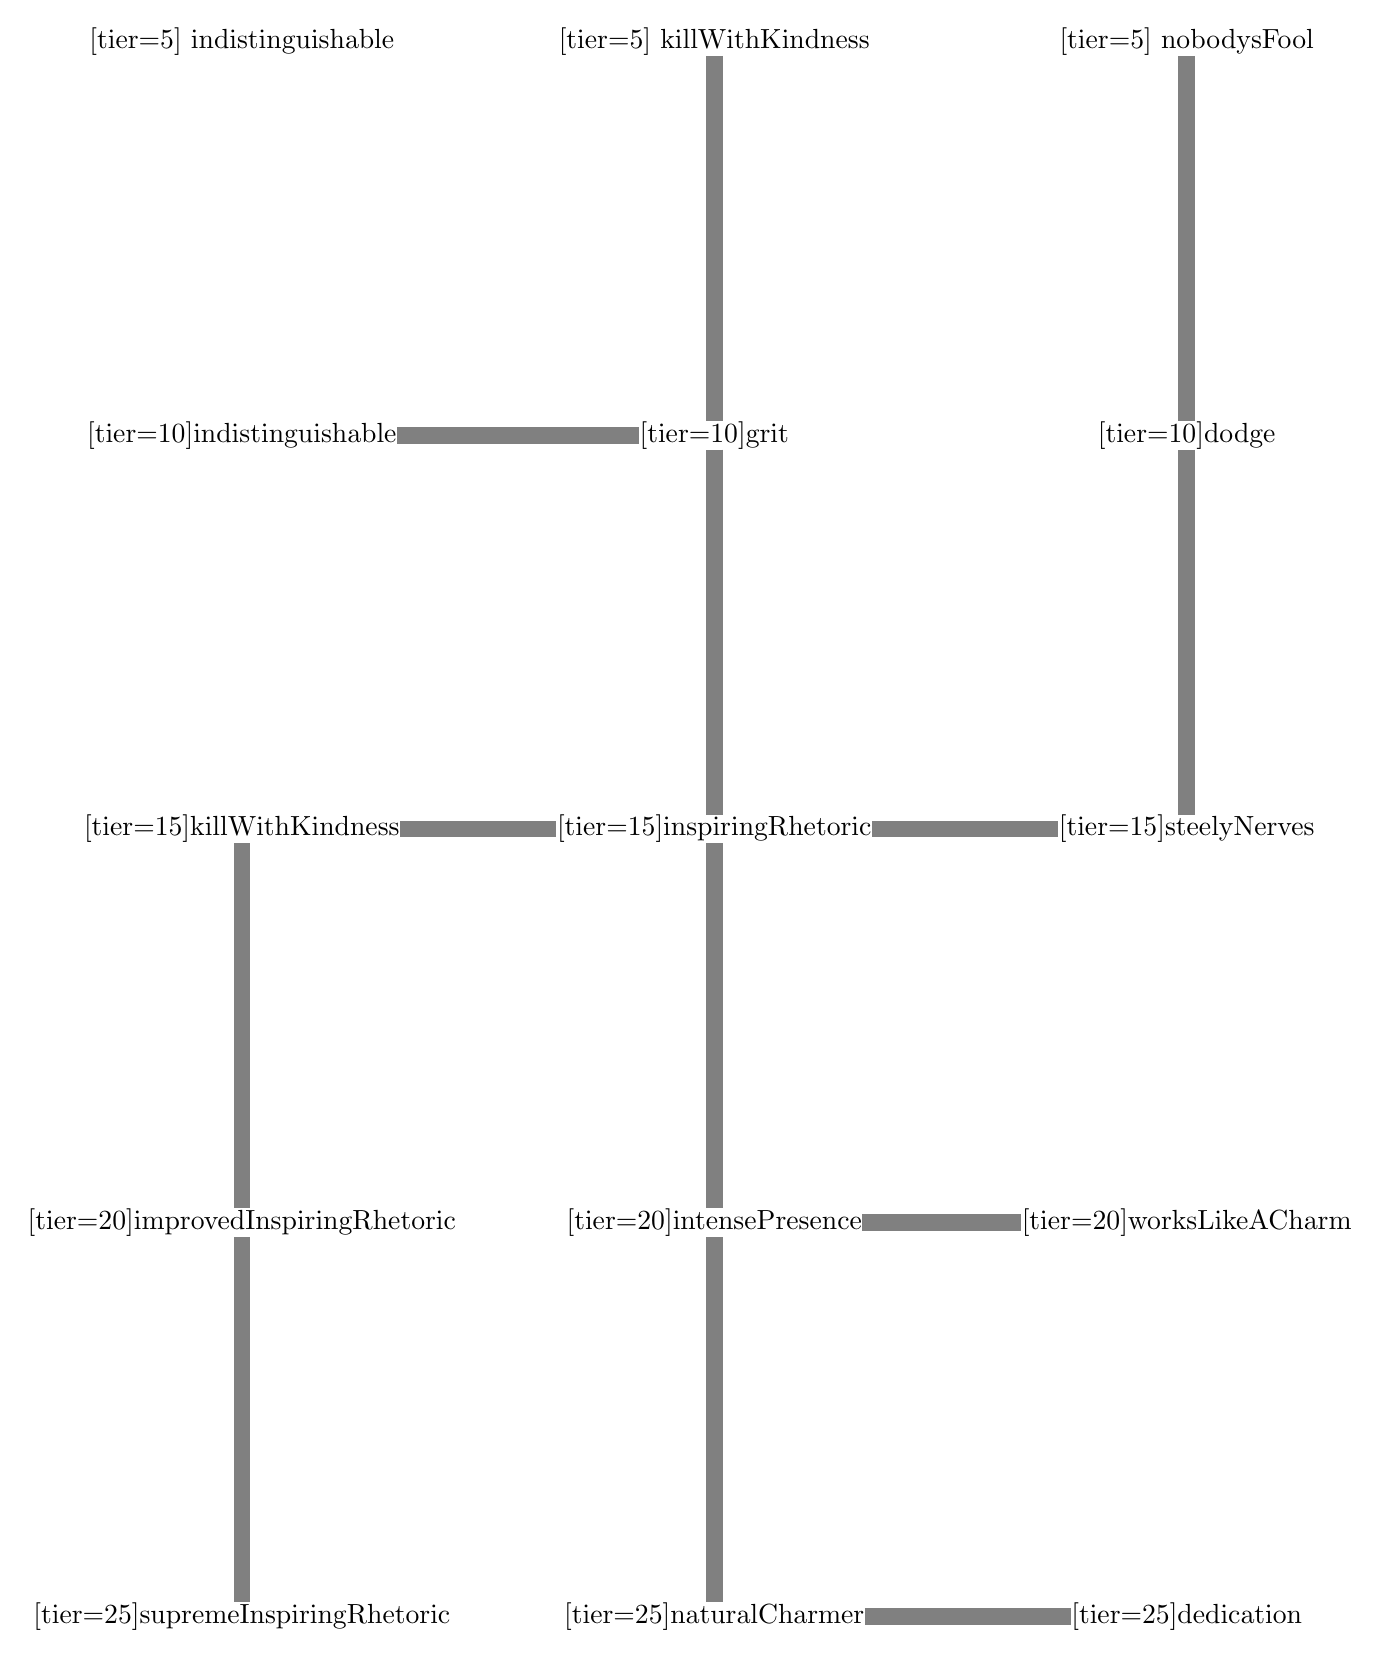
\begin{tikzpicture}
        \draw ( 0,  0) node(aa)[inner sep=0]{\TalentBox[tier=5] {indistinguishable}}
              ( 6,  0) node(ab)[inner sep=0]{\TalentBox[tier=5] {killWithKindness}}
              (12,  0) node(ac)[inner sep=0]{\TalentBox[tier=5] {nobodysFool}}
              ( 0, -5) node(ba)[inner sep=0]{\TalentBox[tier=10]{indistinguishable}}
              ( 6, -5) node(bb)[inner sep=0]{\TalentBox[tier=10]{grit}}
              (12, -5) node(bc)[inner sep=0]{\TalentBox[tier=10]{dodge}}
              ( 0,-10) node(ca)[inner sep=0]{\TalentBox[tier=15]{killWithKindness}}
              ( 6,-10) node(cb)[inner sep=0]{\TalentBox[tier=15]{inspiringRhetoric}}
              (12,-10) node(cc)[inner sep=0]{\TalentBox[tier=15]{steelyNerves}}
              ( 0,-15) node(da)[inner sep=0]{\TalentBox[tier=20]{improvedInspiringRhetoric}}
              ( 6,-15) node(db)[inner sep=0]{\TalentBox[tier=20]{intensePresence}}
              (12,-15) node(dc)[inner sep=0]{\TalentBox[tier=20]{worksLikeACharm}}
              ( 0,-20) node(ea)[inner sep=0]{\TalentBox[tier=25]{supremeInspiringRhetoric}}
              ( 6,-20) node(eb)[inner sep=0]{\TalentBox[tier=25]{naturalCharmer}}
              (12,-20) node(ec)[inner sep=0]{\TalentBox[tier=25]{dedication}}
        ;

        \tikzstyle{bar}=[gray,-,>=stealth, line width=6pt]

        \draw [bar] (ab) to (bb);
        \draw [bar] (ac) to (bc);

        \draw [bar] (bb) to (cb);
        \draw [bar] (bc) to (cc);

        \draw [bar] (ca) to (da);
        \draw [bar] (cb) to (db);

        \draw [bar] (da) to (ea);
        \draw [bar] (db) to (eb);

        \draw [bar] (ba) to (bb);

        \draw [bar] (ca) to (cb);
        \draw [bar] (cb) to (cc);

        \draw [bar] (db) to (dc);

        \draw [bar] (eb) to (ec);
    \end{tikzpicture}
}
